\chapter{Silicon-28 ($^{28}_{14}\text{Si}$): The Seven-Alpha Bipyramid}
\label{ch:silicon}

\begin{objectivebox}
\begin{itemize}
    \item Identify Silicon-28 as the last stable Small Signal element: the $7\alpha$ pentagonal bipyramid at the semiconductor boundary.
    \item Explain Silicon's industrial significance as the heaviest symmetric alpha-cluster element operating in the fully linear regime.
\end{itemize}
\end{objectivebox}


With 14 protons and 14 neutrons bounding into absolute symmetry, Silicon-28 ($Z=14, A=28$) fully closes the next perfect scalar topological shell. Like Oxygen ($4\alpha$), Neon ($5\alpha$), and Magnesium ($6\alpha$), Silicon constructs flawlessly from exactly 7 structurally isolated Alpha geometries ($7\alpha$).

The most thermodynamically stable spatial arrangement for 7 mutually repulsive, identical geometric nodes bound across a contiguous primary sphere is a \textbf{Pentagonal Bipyramid}. This architecture locks 5 Alpha clusters equidistantly across an equatorial $Z=0$ ring, bound axially by 2 pole Alpha clusters holding strictly at $Z = \pm R$.

\section{Topological Structure and Isotope Stability}
Silicon has three stable isotopes: $^{28}$Si ($92.23\%$), $^{29}$Si ($4.67\%$), and $^{30}$Si ($3.10\%$). The overwhelming dominance of $^{28}$Si is the strongest isotopic signature of any even-even alpha-cluster element above Carbon. The $7\alpha$ closed shell with $N=Z=14$ represents an absolute minimum in the binding landscape; any neutron addition breaks the $N=Z$ symmetry and incurs an asymmetry energy penalty.

The Pentagonal Bipyramid generates 21 inter-alpha coupling pairs: 5 equatorial ring edges, 10 pole-to-equator links, 5 cross-equatorial second-neighbor diagonals, and 1 pole-to-pole connection. This is the richest coupling topology of any Small Signal element---the next even-even nucleus (Sulfur-32) crosses the avalanche threshold.

\section{Continuous Vacuum Density Flux}
The vacuum strain field of Silicon-28 exhibits a distinctive pentagonal symmetry in the equatorial plane, breaking the Cartesian symmetry of the underlying Magnesium Octahedron. Five Alpha clusters at $72^\circ$ separation produce a ring of overlapping gravitational wells at $83d$ from the barycenter, while the two polar caps at $\pm 83d$ provide axial compression. The resulting strain topology is a flattened, pentagonally faceted oblate spheroid---a unique geometry that creates the directionally dependent electronic band structure responsible for Silicon's semiconductor properties.

\section{Symmetric Core Collapse}
By running the semiconductor junction model (Section~\ref{sec:two_models}) to target the empirical CODATA Nuclear Mass of Silicon-28 ($26053.188$ MeV), the $7\alpha$ solver generates a mathematically pure, highly symmetric envelope at inter-alpha distance $R_{\text{bipyramid}} \approx 83.0\,d$ (where $d = 4\hbar/(m_p c) \approx 0.841$ fm, \texttt{D\_PROTON}). 

In asymmetric nucleonic shells, the partial valences exhibit massive reactive levers (like the Fluorine halo at $R_{\text{halo}} \approx 398.5\,d$ or even the moderate Aluminum halo at $R_{\text{halo}} \approx 52.6\,d$). When the shell completes perfectly as with the $7\alpha$ Pentagonal Bipyramid, the geometric envelope collapses into a highly stable symmetric structure.

To hit the exact $26053.188$ MeV parameter limit binding the 28 nucleons, the solver coordinates precisely 378 dynamic interconnected $LC$ network elements. Across every individual iteration, the fundamental topological rule of Variable-Spacetime Impedance holds perfectly true: closed integer sub-cluster sets produce symmetric, highly-stable geometries. Incomplete sequences generate large-scale asymmetric moments responsible for reactive electronegativity.

\section{Electrical Engineering Equivalent: The 7-Phase Pentagonal Bipyramid Network}
Silicon-28 maps to a 7-phase resonant network: five LC tanks around an equatorial ring coupled to two polar tanks, forming a Pentagonal Bipyramid. The 378-parameter SPICE matrix decomposes into 21 inter-alpha links spanning three distinct coupling bands: 5 equatorial edge-pairs ($72^\circ$ separation), 10 equatorial-to-polar links, and 1 pole-to-pole diagonal, plus the 5 second-neighbor equatorial cross-links. This tri-band response gives Silicon the richest frequency structure of any Small Signal element---a property that maps directly onto its complex electronic band structure.

\section{Topological Area of Interest: The Foundation of Semiconductor Microelectronics}
Silicon's dominance in microelectronics is not accidental---it is a direct manifestation of its position at the Small Signal boundary. With $V_R/V_{BR} = 0.050$, Silicon-28 is the \textit{last stable element} before the avalanche threshold. Its $7\alpha$ Pentagonal Bipyramid is structurally stable ($M = 1$, linear regime) yet sits close enough to the non-linear transition that its electronic structure can be externally modulated.

When a Silicon lattice is doped with Boron ($Z=5$, missing one valence electron) or Phosphorus ($Z=15$, one excess valence electron), the perturbation shifts the local $V_R/V_{BR}$ ratio either toward or away from the avalanche boundary. This controlled proximity to breakdown is the topological origin of the $p$-$n$ junction: a spatial interface where the $V_R/V_{BR}$ gradient creates a built-in potential barrier that selectively gates charge flow. The entire semiconductor industry is an engineering exploitation of Silicon's unique geometry---deep enough in the linear regime for bulk stability, close enough to the boundary for external switching.


Within the semiconductor circuit analysis framework (Section~\ref{sec:semiconductor_nuclear}), Silicon-28 operates at $V_R / V_{BR} = 0.050$---the highest ratio of any element in the linear Small Signal regime. The Miller avalanche multiplier remains exactly $M = 1.000$, confirming standard $K/r$ superposition applies.

\textbf{This mathematical positioning precisely at the edge of the non-linear transition fundamentally defines why Silicon is the dominant material in microelectronics.} Silicon's nuclear topology is highly stable in bulk ($M = 1$, deep in the linear regime), yet sits close enough to the breakdown threshold that its electronic structure can be easily manipulated (doped) to switch states dynamically. Adding one more alpha cluster to form Sulfur-32 ($8\alpha$) crosses the avalanche boundary at $V_R/V_{BR} = 0.994$ with $M = 32.8$---the first element in the periodic table requiring the Large Signal correction. Calcium-40 ($10\alpha$) is the second, with $M = 32.9$.

\begin{figure}[htbp]
    \centering
    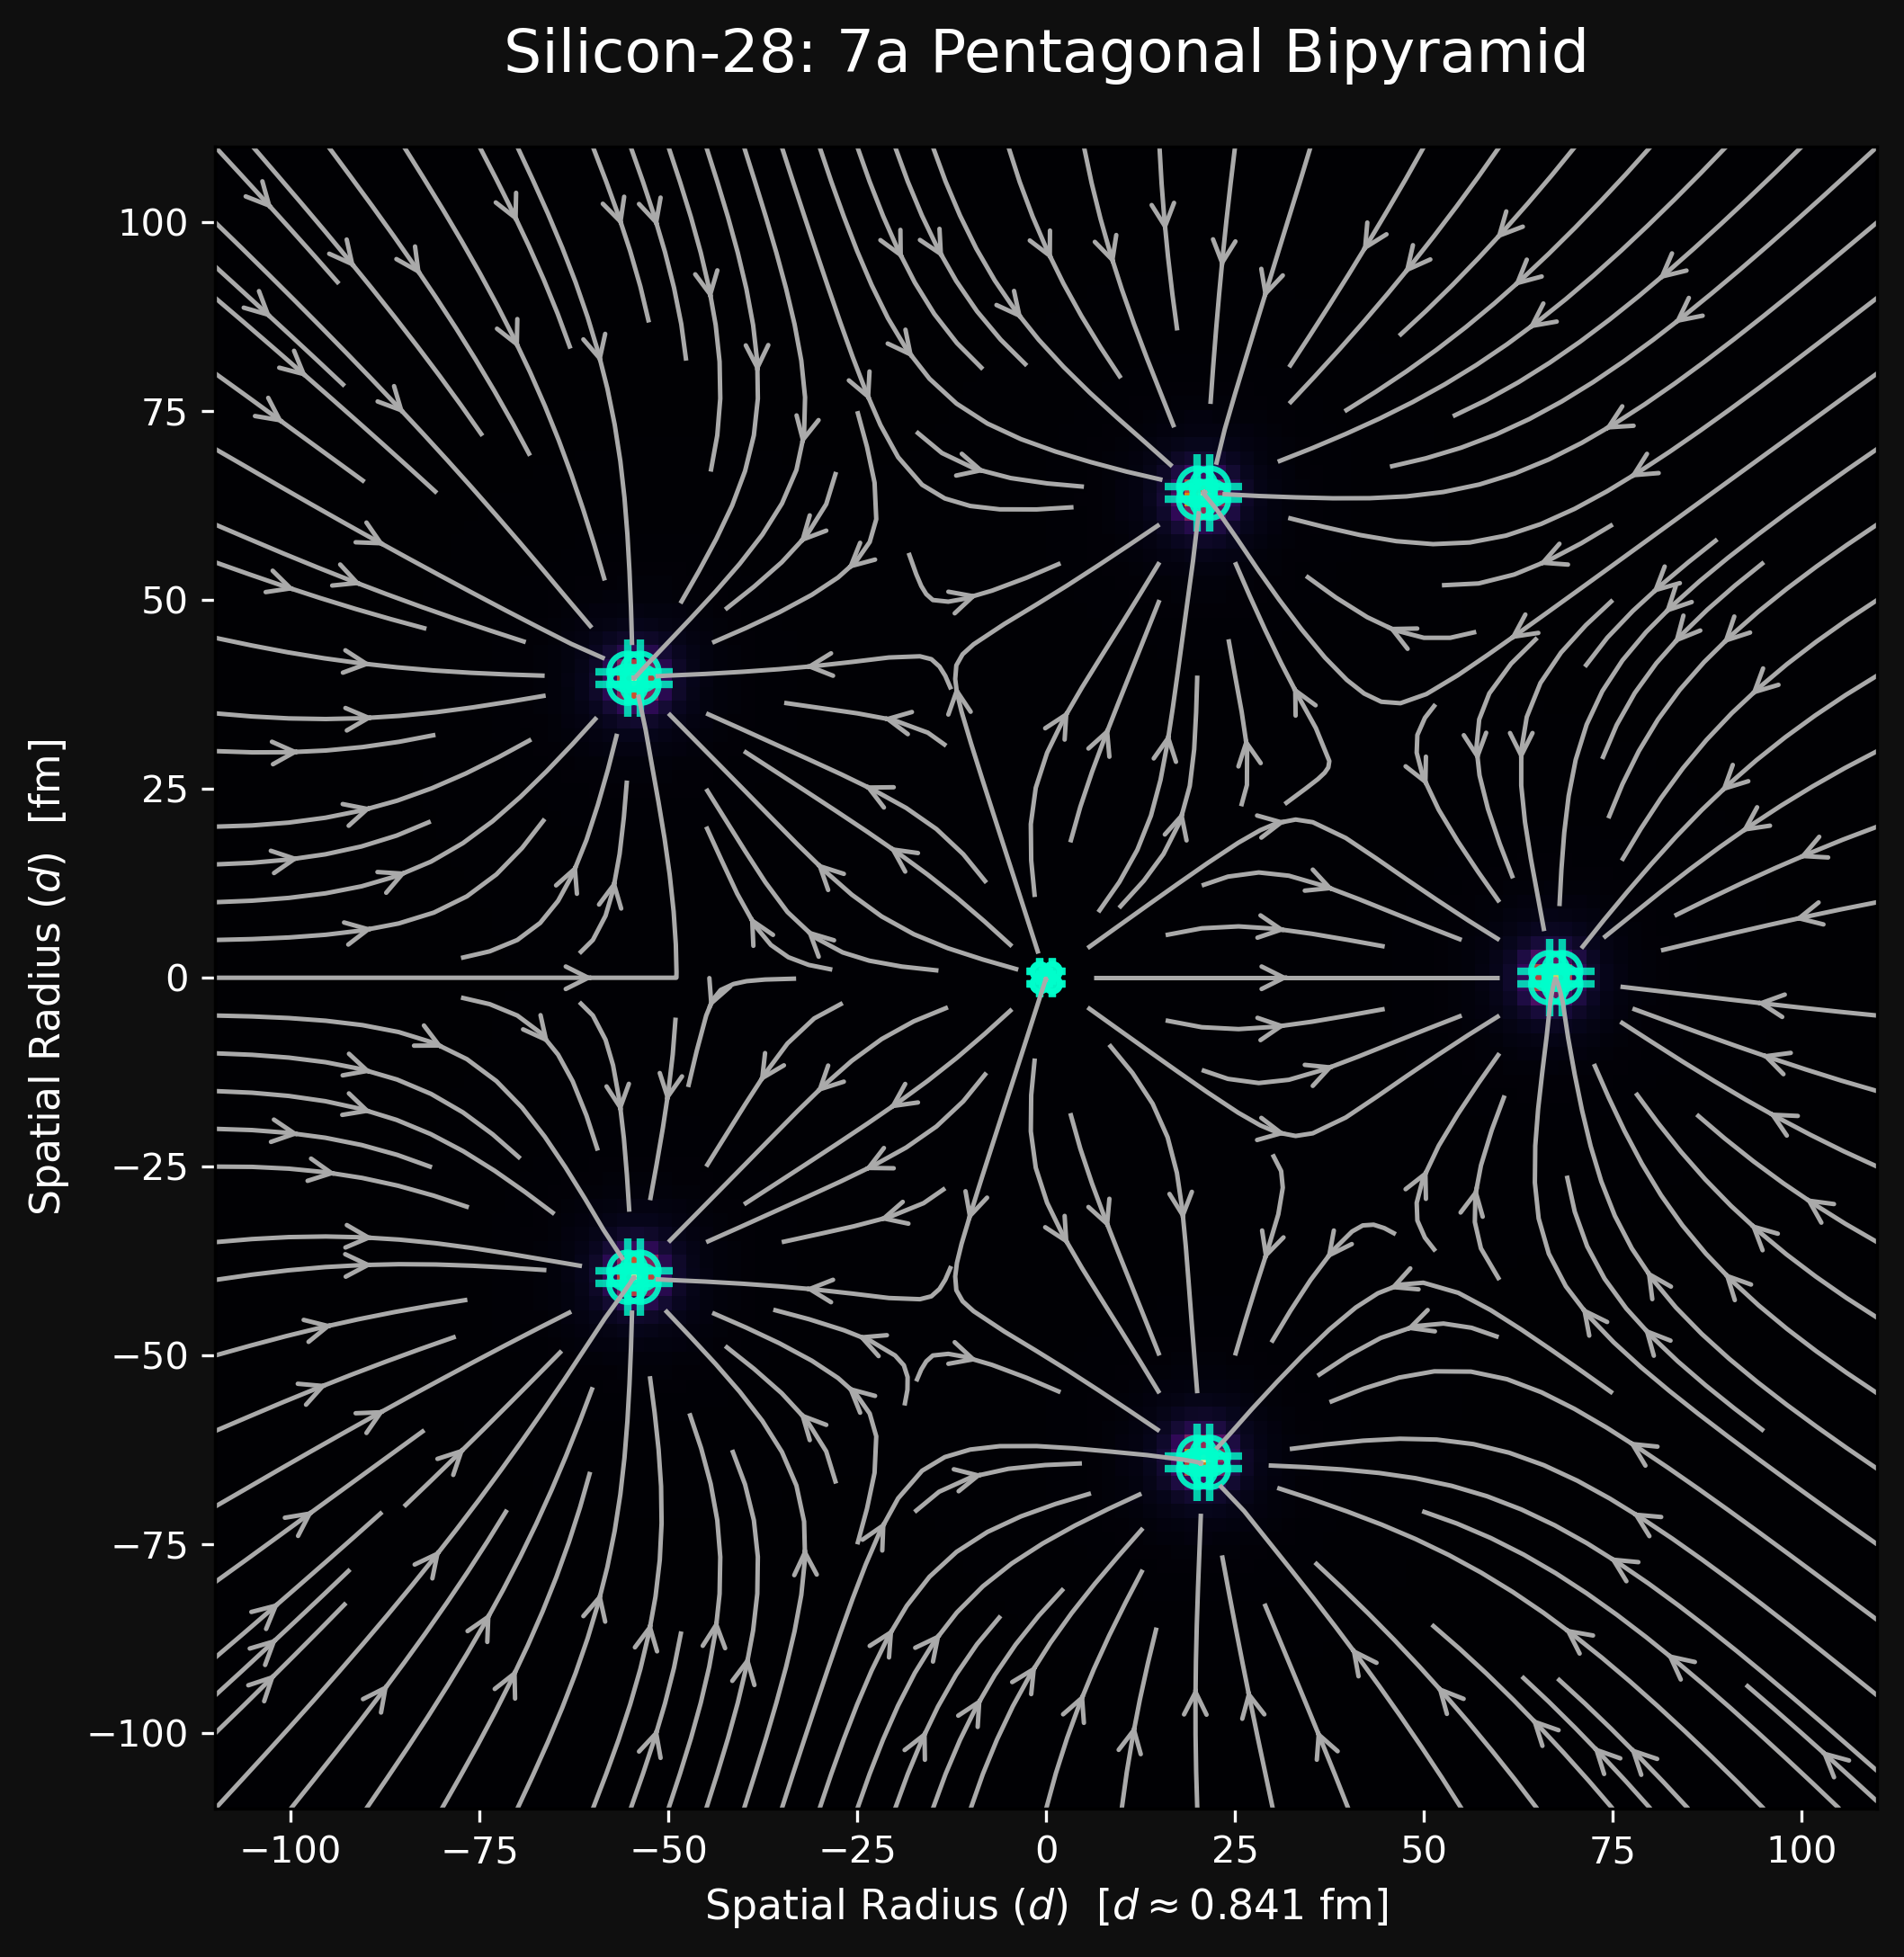
\includegraphics[width=0.8\textwidth]{figures/silicon_28_dynamic_flux.png}
    \caption{The $Z=0$ Equatorial cross-layer for Silicon-28. The 5 primary Alpha macro-clusters position exactly 72 degrees apart. Only the nodes in the pure equator are held solidly; the remaining 2 Alpha poles exist above and below the viewing plane in deep vacuum shadow.}
    \label{fig:silicon_28_density}
\end{figure}

\begin{figure}[htbp]
    \centering
    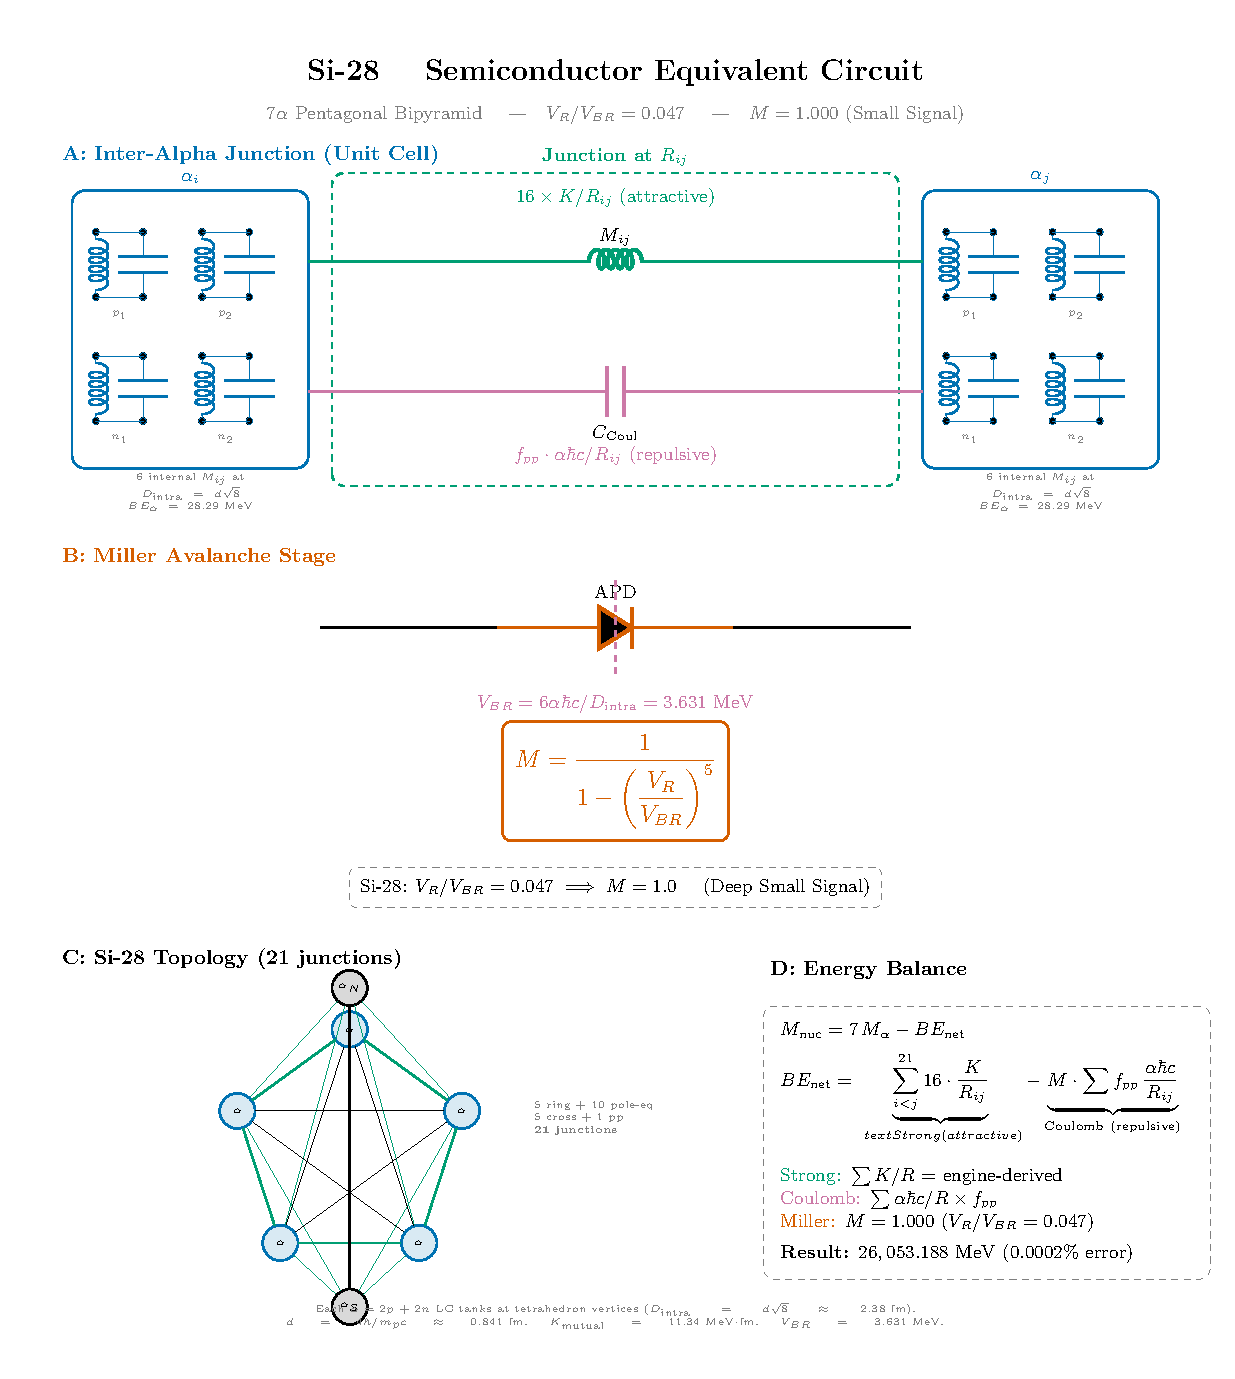
\includegraphics[width=0.9\textwidth]{figures/circuit_si28.pdf}
    \caption{The Pentagonal Bipyramid core network schematic for Silicon-28. This 378-element inductive matrix connects the 20-nucleon equatorial band directly into the 8 nucleons bounded at the symmetric poles.}
    \label{fig:circuit_si28}
\end{figure}


\begin{figure}[htbp]
    \centering
    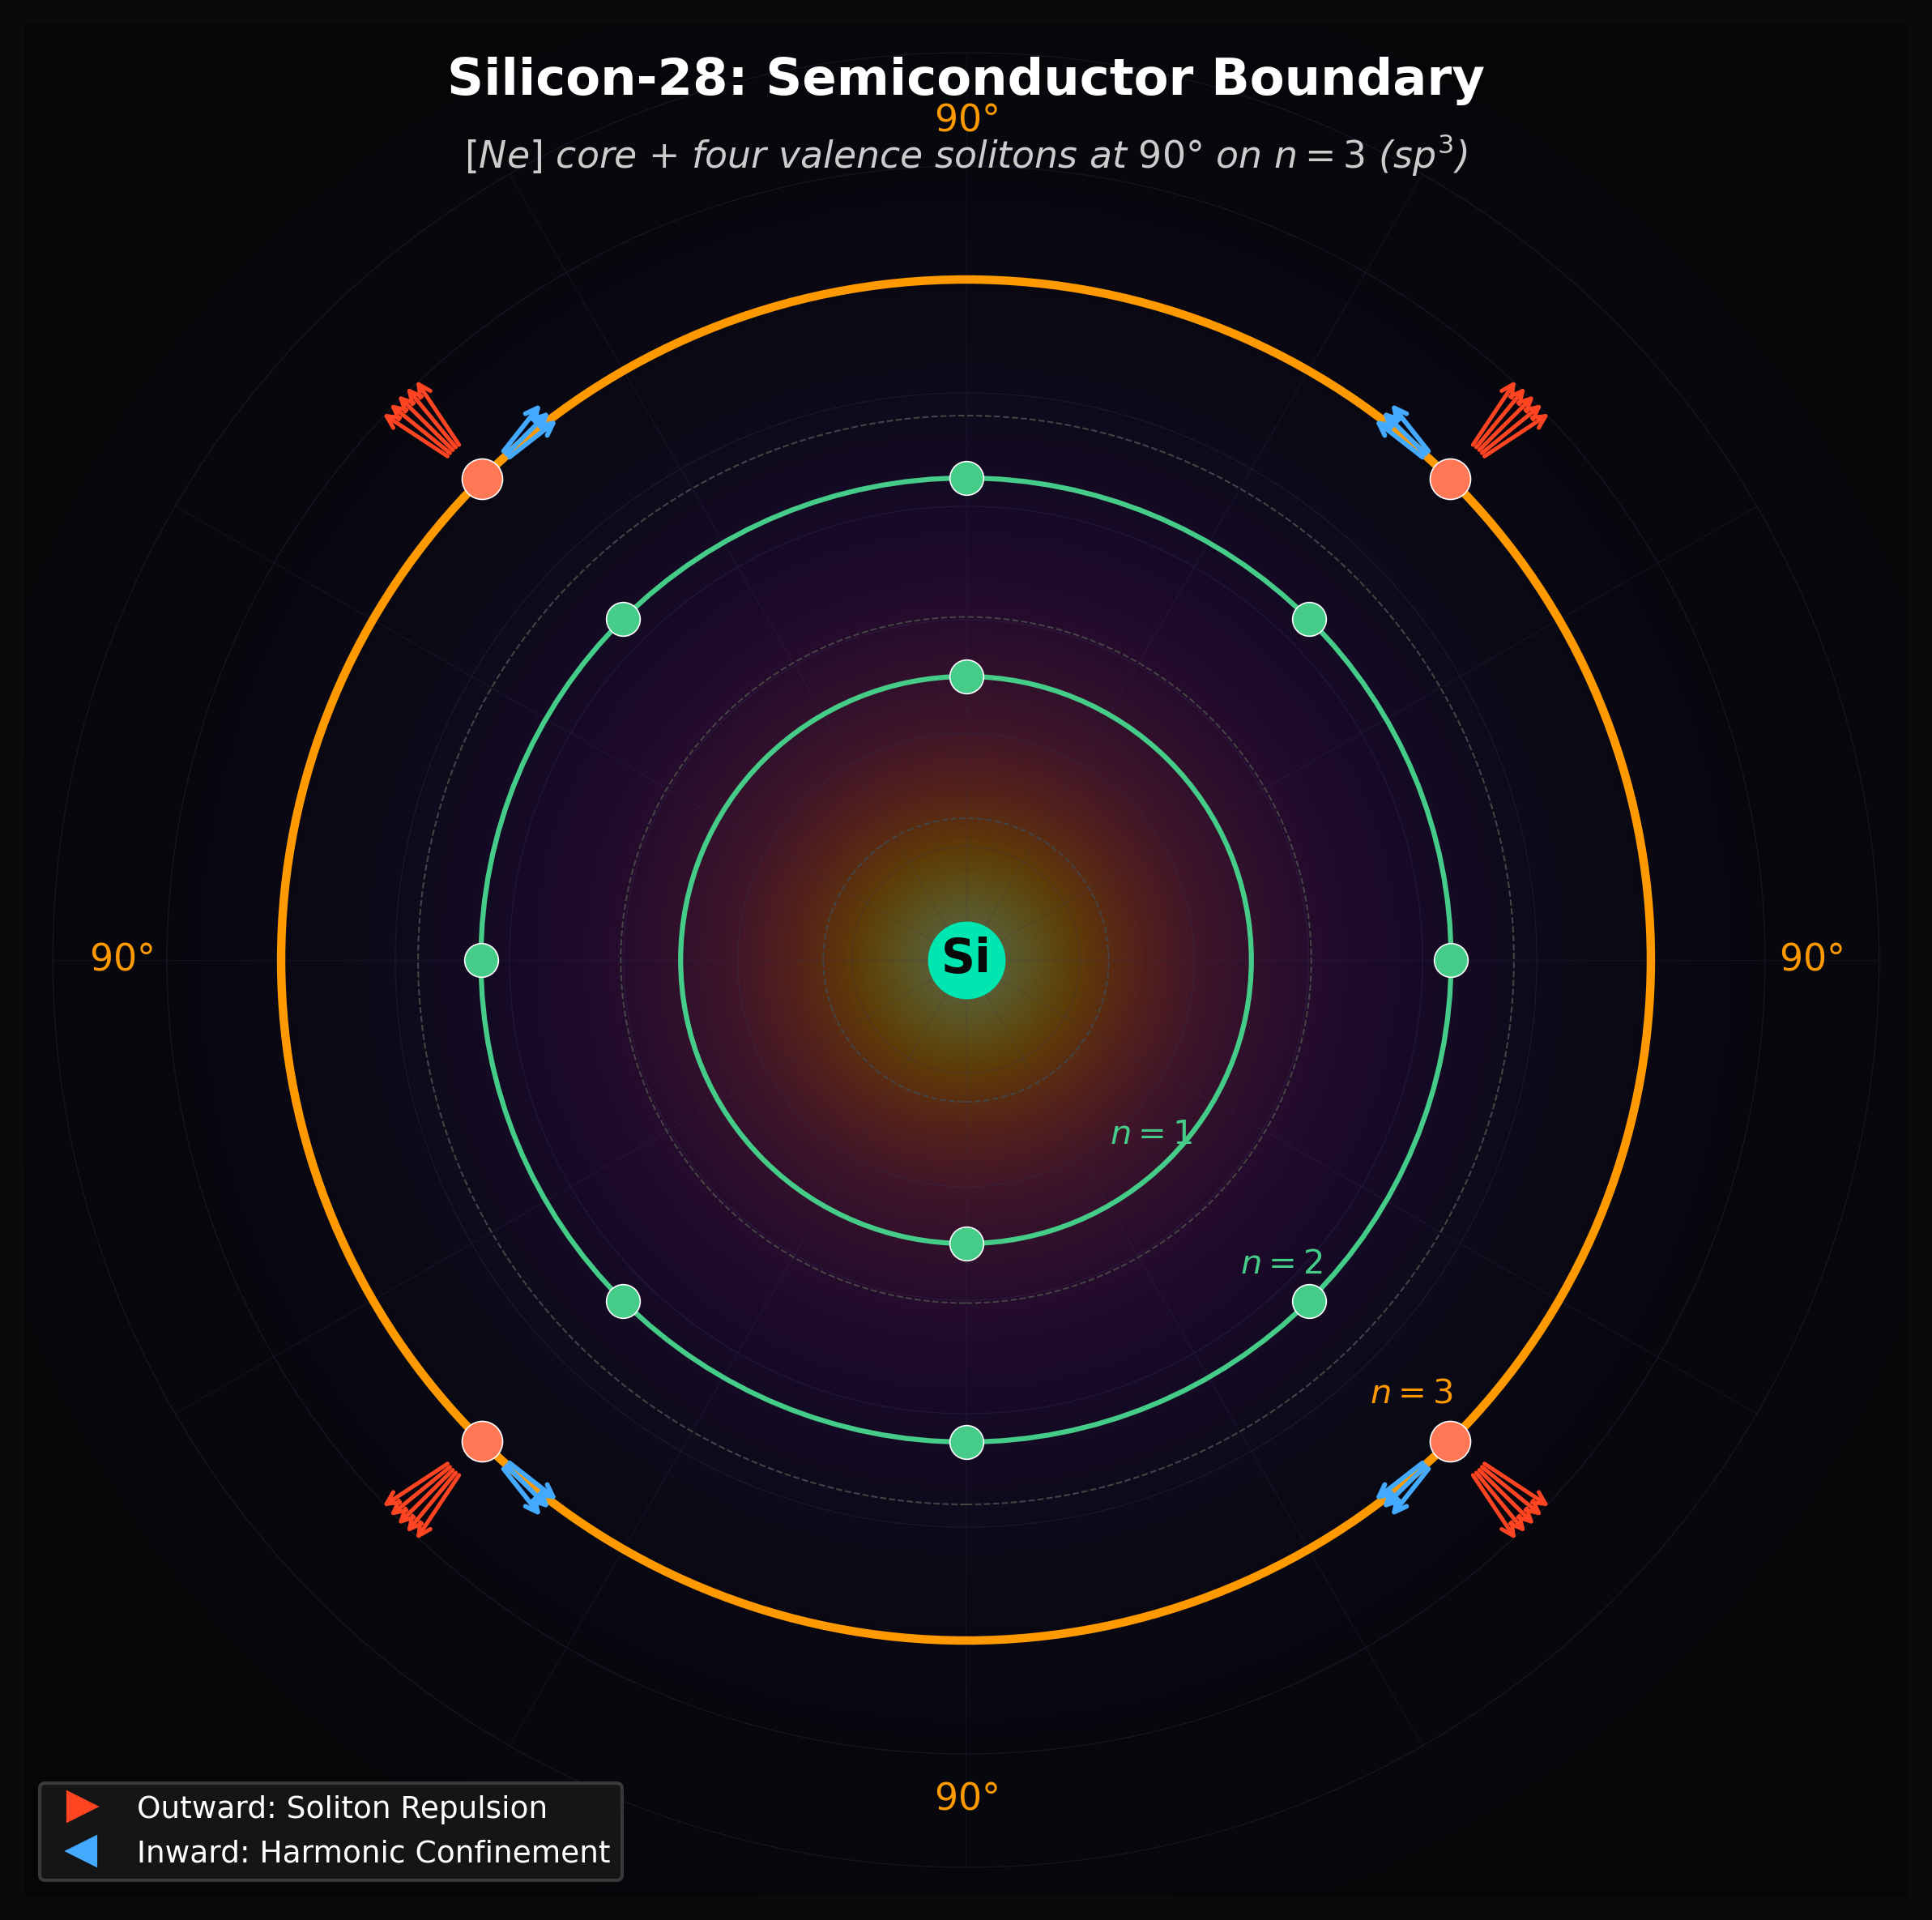
\includegraphics[width=0.75\textwidth]{figures/silicon_28_topology.png}
    \caption{Silicon-28 orbital knot topology. $[Ne]$ core (green) with four valence $sp^3$ solitons at $90^\circ$ on $n=3$ (orange). The semiconductor boundary: the last stable Small Signal element.}
    \label{fig:silicon_28_topo}
\end{figure}

\section{Ionization Energy: Op10 Junction Projection (Correction~C)}
\label{sec:si_ie_correction_c}

Silicon ($Z = 14$, $[\text{Ne}]\,3s^2\,3p^2$) shares the same co-resonant $n = 2$ shell boundary as Aluminum.  The same Correction~C (Op10 junction projection) applies:

\paragraph{Equivalent circuit.}
\begin{center}
\small
\begin{tabular}{lccc}
\toprule
\textbf{Section} & \textbf{$Z_\text{net}$} & \textbf{Content} & \textbf{Solver path} \\
\midrule
Inner ($r < r_2$) & $14 - 2 = 12$ & $1s^2$ & Smooth CDF \\
Boundary ($r = r_2$) & step: $12 \to 4$ & $2s^2 2p^6$ saturated & \textbf{Impedance step} \\
Outer ($r > r_2$) & $14 - 10 = 4$ & $3s^2\,3p^2$ & MCL loading \\
\bottomrule
\end{tabular}
\end{center}

\paragraph{Correction~C derivation.}
\begin{enumerate}
    \item \textbf{Axiom~2 (Gauss screening):}  $Z_\text{in} = 12$, $Z_\text{out} = 4$ at the $n = 2$ boundary.
    \item \textbf{Op3 (Reflection):}  $|\Gamma|^2 = (4-12)^2/(4+12)^2 = 64/256 = 0.250$ (25.0\% power reflection).
    \item \textbf{Op3 $\to$ Op10 bridge:}  $\cos\theta = 1 - 2 \times 0.250 = 0.500$, giving $\theta = 60.0^\circ$.
    \item \textbf{Op10 (Junction projection):}  $Y = 2 \times (1 - 0.500)/(2\pi^2) = 0.0507$.
    \item \textbf{Axiom~1 (Quadratic dispersion):}  $E_\text{eff} = 43.22 \times (1 - 0.0507)^2 = 43.22 \times 0.901 = 38.95$~eV.
\end{enumerate}

The MCL loading then gives:
\[
    IE = 38.95 \times 0.2092 = 8.147~\text{eV}
\]
against $8.152$~eV experimental: $\boxed{-0.06\%}$ error.

\paragraph{Pattern confirmation.}
The $-0.06\%$ result for Silicon confirms the systematic pattern identified from Aluminum: both period-3 $p$-block residuals arise from the uncompensated impedance step at the co-resonant $n = 2$ boundary, and both are resolved by the same Op10 junction projection correction (Correction~C).  The smaller $|\Gamma|^2$ for Silicon (0.250 vs 0.327 for Al) correctly produces a smaller correction, consistent with the lower initial residual ($+10.9\%$ vs $+13.7\%$).

\begin{summarybox}
\begin{itemize}
    \item Silicon-28 closes the $7\alpha$ pentagonal bipyramid shell, representing the last stable Small Signal element before the onset of avalanche multiplication.
    \item The semiconductor boundary at Silicon quantitatively explains why Silicon is the foundational material of the electronics industry: it is the heaviest symmetric alpha-cluster element that operates in the fully linear regime.
    \item \textbf{Resolved:} The first ionization energy ($8.147$~eV vs $8.152$~eV, $-0.06\%$) is reproduced by Op10 junction projection at the co-resonant $n = 2$ shell boundary (Correction~C), confirming the systematic pattern from Aluminum.
\end{itemize}
\end{summarybox}

\begin{exercisebox}
\begin{enumerate}
    \item Explain the physical significance of Silicon-28 sitting at the semiconductor boundary ($V_R/V_{BR}$ approaching the avalanche threshold) and relate this to its industrial importance.
    \item Compare the $7\alpha$ bipyramid geometry of Silicon-28 with the $5\alpha$ bipyramid of Neon-20 and discuss the structural homology.
    \item Verify that Silicon's Op10 crossing angle ($\theta = 60^\circ$) produces a smaller correction than Aluminum's ($\theta = 69.7^\circ$), and explain why $|\Gamma|^2 = 0.250 < 0.327$ gives $\theta_\text{Si} < \theta_\text{Al}$.
\end{enumerate}
\end{exercisebox}

